\subsubsection{Scénario Cockburn}
\textbf{Cas d'utilisation:} Payer par carte

\textbf{Acteur primaire:} Le conducteur

\textbf{Pré-condition: } La borne accepte le payement par carte.
 
\textbf{Post-condition: }  La transaction a été acceptée ou pas.

\textbf{Scenario primaire: } \\
    \textbf{1.} Le conducteur insère sa carte. \\
    \textbf{2.} Le lecteur détecte une carte bleue. \\
    \textbf{3.} Le lecteur effectue un paiement par carte bleue.\\
    \textbf{4.} Le conducteur récupère sa carte.\\

\textbf{Variantes:}\\
    \textbf{2a1.} Le lecteur détecte une carte d’abonnement.\\
    \textbf{2a2.} Le lecteur effectue un paiement par abonnement. Aller en 4.\\
    \textbf{2b.} Le lecteur détecte une carte non valide.  Aller en 4. \\
    
\newpage
\subsubsection{Diagramme d'activité}
\begin{figure}[h]
    \centering
    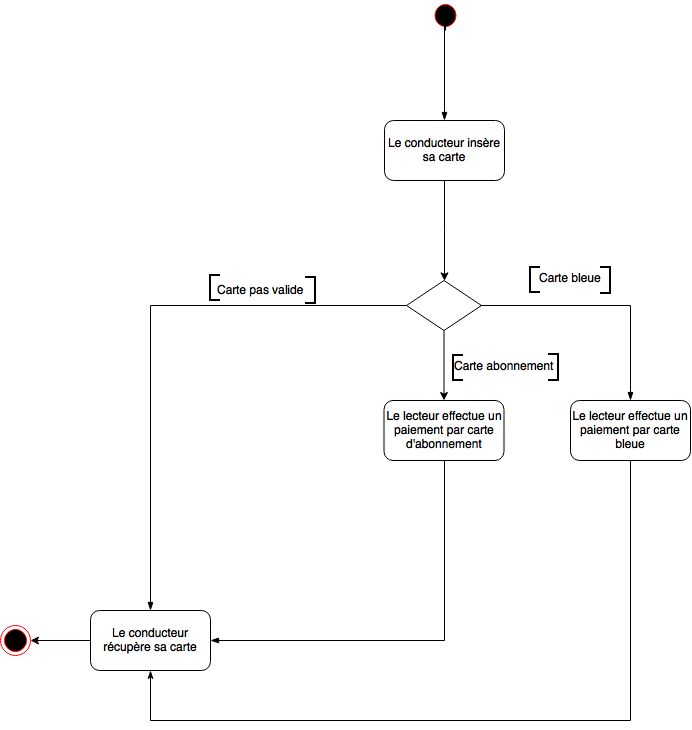
\includegraphics[scale=0.45]{02_Desenvolvimento/TD2/images/DA-PayerCarte.png}
    \caption{Diagramme d'activité: Payer par carte}
\end{figure}
\newpage
\subsubsection{Collaboration}
\begin{figure}[h]
    \centering
    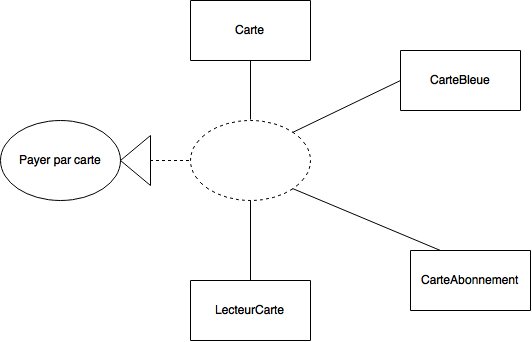
\includegraphics[scale=0.6]{02_Desenvolvimento/TD2/images/ColaCarte.png}
    \caption{Collaboration: Payer par carte}
\end{figure}